\documentclass[12pt,a4paper,english,nofootinbib,sort&compress,numbers]{revtex4-2} % Defines the basic parameters of the document
% If you want a doubble-column, add "reprint"

% Allows special characters (including æøå)
\usepackage[utf8]{inputenc}

% It may be usefult to download TeXMaker, because it includes a large library of the most common packages.

\usepackage{physics,amssymb}  % mathematical symbols (physics imports amsmath)
\usepackage{amsmath}          %Allows usage of mathematical expressions
\usepackage{graphicx}         % include graphics such as plots
\graphicspath{ {Images/} }

\usepackage{xcolor}           % set colors
\usepackage{hyperref}         % automagic cross-referencing
\usepackage{listings}         % display code

\usepackage{algorithm}        % structure and display algorithms
\usepackage[noend]{algpseudocode} % environment to write pseudocode
\usepackage{float}            % make sure that algorithms float with revtex4-2
\usepackage{tikz}             % for creating graphics
% Defines the color of hyperref objects
% Blending two colors:  blue!80!black  =  80% blue and 20% black
\hypersetup{ % this is just my personal choice, feel free to change things
    colorlinks,
    linkcolor={red!50!black},
    citecolor={blue!50!black},
    urlcolor={blue!80!black}}


\usepackage{caption}          %Allows usage of plots
\usepackage{subcaption}       %Allows usage of subplots

\newcommand{\iris}[1]{\textbf{\textcolor{blue}{#1}}}
\newcommand{\jonas}[1]{\textbf{\textcolor{red}{#1}}}
\newcommand{\larsmartin}[1]{\textbf{\textcolor{green}{#1}}}

\newcommand{\nl}{\bigskip\noindent}


\begin{document}
% ===========================================
% Title and authors
\title{FYS-STK4155 Project 3 \\ }       
\author{Lars-Martin Gihle, Iris Bore \& Jonas Båtnes   \\ \textit{University of Oslo, Department of Physics}}        % Sets the author's name.
\date{\today}                  % Sets the document date.

% ===========================================

\noaffiliation                 % Ignore this, but keep it.

\begin{abstract}
    
\end{abstract}

\maketitle

% ===========================================
\section{Abstract}
%
\label{sec:Abstract}
With the rise of artificial neural networks enabled by improved computational resources, optimizing models for specific tasks has become crucial. Convolutional Neural Networks (CNNs) excel in image classification, proving valuable in applications such as autonomous driving and diagnostics. In this study, we perform a grid search across the number of nodes, layers, and activation functions to optimize digit classification on the MNIST dataset. We highlight the impact of different pooling layer implementations on performance and compare CNN results to logistic regression models implemented with PyTorch. By testing various hyper parameters, the logistic regression model achieves an accuracy of 92\% \iris{check this on test set again}, significantly lower than the 99\% accuracy of the CNN.

% ===========================================
% ===========================================
\newpage
\section{Introduction}
%
\label{sec:introduction}
In recent years, convolutional neural networks (CNNs) have emerged as a cornerstone technology in computer vision and broader industrial applications, powering innovations in areas such as autonomous vehicles, facial recognition, and quality inspection \cite{lecun2015deep, krizhevsky2012imagenet}. By leveraging convolutional layers to capture local spatial patterns, pooling operations to reduce dimensionality, and fully connected layers to integrate learned features, CNNs have demonstrated exceptional performance across a wide range of classification, detection, and segmentation tasks \cite{he2016deep}. Their capacity to automatically learn hierarchical features from raw input data makes them particularly well-suited for complex image-based challenges.

In parallel, classical approaches such as Linear Regression offer a useful baseline for understanding dataset complexity and benchmarking the performance gains afforded by more sophisticated neural architectures \cite{hastie2009elements}. While Linear Regression alone is not typically suited for image classification, comparing it against CNNs helps illuminate the advantages of nonlinear feature extraction and deep representation learning. To further explore the performance of Linear Regression on classification tasks, we experiment with multiple hyperparameters. Specifically, we test five distinct learning rates, batch sizes, and numbers of epochs to assess how these variations influence the model's classification accuracy and convergence behavior.

In this study, we focus on the well-known MNIST dataset, a benchmark collection of handwritten digit images that serves as a standardized platform for evaluating classification models \cite{lecun1998gradient}. We employ a systematic approach to hyperparameter optimization by conducting a comprehensive grid search over CNN architectures and their key hyperparameters. By exploring various configurations—such as differing numbers of convolutional filters, kernel sizes, and network depths—we aim to identify the CNN architecture that yields the best classification accuracy on MNIST.

Our evaluation metrics center on classification accuracy, allowing us to directly compare the predictive power of our best-performing CNN against the Linear Regression models tested under varying learning rates, batch sizes, and epoch counts. We also discuss the computational considerations associated with both approaches, as modern industrial applications often require methods that are both accurate and efficient.

This article is structured as follows: we begin by introducing the MNIST dataset and detailing the preprocessing steps taken to ensure data quality and consistency. We then outline the architectural components of CNNs and the rationale behind their effectiveness in image classification tasks. Following this, we describe the grid search procedure employed to explore the hyperparameter space of CNN architectures and linear configurations. We next define our baseline Linear Regression model and the variations introduced in learning rates, batch sizes, and epochs to investigate their impact on performance. Subsequently, we present and analyze the results, highlighting how different CNN architectures and hyperparameters compare against the various Linear Regression configurations. Finally, we summarize our findings, discuss their implications for real-world industrial contexts, and suggest avenues for future researchs.

% ===========================================
\newpage
\section{Methods}\label{sec:methods}
%
\label{sec:methods}
This study primarily focused on implementing and comparing the performance of various Convolutional Neural Networks (CNNs) with different layers, kernel sizes, filter numbers, and activation functions on the MNIST dataset. To illustrate the advantages of CNNs, we benchmarked our results against Logistic Regression (LR) across five different learning rates, batch sizes, and epochs. To ensure the robustness and reliability of our findings, we employed several data preprocessing and optimization techniques, including train-test splitting, cross-validation on the training set, and bootstrapping on the test set.                


\subsection{Data Loading and Preprocessing}

\subsubsection{Train-Test Split}

We used PyTorch to load the MNIST dataset, which comprises 70,000 images in total. This dataset is pre-divided into a training set of 60,000 images and a test set of 10,000 images. During the optimization process, the training set was utilized to iteratively update the model parameters in order to minimize the loss function. Meanwhile, the test set remained completely untouched until the final evaluation phase. This separation allowed us to evaluate the model's ability to generalize to new, unseen data. By conducting model selection and hyperparameter tuning exclusively on the training data, and reserving final performance checks for the test data, we obtained a more realistic measure of the model’s predictive power and robustness.

\subsubsection{Feature Scaling}

Given that our dataset is composed of pixels confined to a specific range, we relied on Raschka's perspective that scaling the MNIST dataset was unnecessary \cite{raschka2022machine}. Although we have consistently scaled our data in the previous projects, our primary goal for this project was to optimize parameters through cross-validation on the training data. To prevent data leakage between folds and to reduce the computational costs associated with scaling within each fold, we decided not to scale the data.

\subsection{Classification Techniques}

The following classification methods were implemented:

\subsubsection{Convolutional Neural Network}

Convolutional Neural Networks are a type of deep learning model specifically designed for processing structured grid data, such as images. CNNs exploit spatial hierarchies in data by applying convolutional operations to extract features. These features are then used to perform classification tasks.

A key component of a CNN is the convolution operation. For a 2D input, the convolution is defined as in equation \ref{eq:CNN2Dinput}:

\begin{equation}
    (f * g)(x, y) = \sum_{m=-\infty}^{\infty} \sum_{n=-\infty}^{\infty} f(m, n) \cdot g(x - m, y - n)
    \label{eq:CNN2Dinput}
\end{equation}

Here, \(f(m, n)\) represents the input image, and \(g(x - m, y - n)\) is the filter or kernel. The kernel slides over the image to compute feature maps.

To control the size of the output feature maps, CNNs often use padding and strides. Padding can increase the dimensionality of the output and as such avoid the shrinking that convolutional layers usually apply to the tensor when passing through them. The size of the output feature map, \(D_{out}\), for an input of size \(D_{in}\), a kernel (filter) size \(K\), stride \(S\), and padding \(P\), is calculated as in equation \ref{eq:outputfeaturemapequation}:

\begin{equation}
    D_{out} = \left\lfloor\frac{D_{in} - K + 2P}{S}\right\rfloor + 1
    \label{eq:outputfeaturemapequation}
\end{equation}

The output tensor is then of dimensions $D_{out}\times D_{out}\times C$ where $C$ is the number of channels. Padding is also useful to help capture more information from edge pixels, since it allows filters to capture edge pixels more times as it slides over the image.
The final layers of a CNN are typically fully connected (dense) layers, which map the extracted features to class probabilities using the softmax function in equation \ref{eq:softmaxfunction}:

\begin{equation}
    p(y = c \mid \boldsymbol{x}) = \frac{\exp(z_c)}{\sum_{k=1}^C \exp(z_k)}
    \label{eq:softmaxfunction}
\end{equation}

Here, \(z_c\) represents the output score for class \(c\), and \(C\) is the total number of classes.

CNNs are trained using backpropagation, where the loss function, such as cross-entropy in equation \ref{eq:Lossfuntion}, guides the optimization of weights:

\begin{equation}
    L = -\sum_{i=1}^n \sum_{c=1}^C y_{i,c} \log \hat{y}_{i,c}
    \label{eq:Lossfuntion}
\end{equation}

In this equation, \(y_{i,c}\) is the true label, and \(\hat{y}_{i,c}\) is the predicted probability for class \(c\).

CNNs have demonstrated exceptional performance in image classification tasks by automatically learning hierarchical features from raw input data \cite{raschka2022machine}.

\subsubsection{Logistic Regression}

Logistic regression can be used for multiclass classification problems, predicting the probability that an input $\boldsymbol{x}_i$ belongs to one of several classes $y_i \in {0, 1, \dots, K-1}$. It models these probabilities using the softmax function in equation \ref{eq:softmaxfunction}, which outputs values between 0 and 1 that sum to 1 across all classes:

\begin{equation}
p(y_i = k \vert \boldsymbol{x}_i, \boldsymbol{\beta}) = \frac{\exp(\boldsymbol{x}_i^\mathrm{T} \boldsymbol{\beta}k)}{\sum{j=0}^{K-1} \exp(\boldsymbol{x}_i^\mathrm{T} \boldsymbol{\beta}_j)}, \quad \text{for } k = 0, 1, \dots, K-1.
\label{eq:softmaxfunction}
\end{equation}

To estimate the parameters $\boldsymbol{\beta}$, Maximum Likelihood Estimation (MLE) is used. Assuming independent data points, the likelihood function for the dataset $\mathcal{D} = { (\boldsymbol{x}_i, y_i) }$ is described in equation \ref{eq:likelihoodfunction_softmax}:

\begin{equation}
L(\boldsymbol{\beta}) = \prod_{i=1}^n \prod_{k=0}^{K-1} [p(y_i = k \vert \boldsymbol{x}_i, \boldsymbol{\beta})]^{\mathbb{1}(y_i = k)},
\label{eq:likelihoodfunction_softmax}
\end{equation}

where $\mathbb{1}(y_i = k)$ is an indicator function that equals 1 if $y_i = k$ and 0 otherwise.

The log-likelihood function is then expressed as in equation \ref{eq:loglikelihoodfunction_softmax}:

\begin{equation}
\ell(\boldsymbol{\beta}) = \sum_{i=1}^n \sum_{k=0}^{K-1} \mathbb{1}(y_i = k) \log p(y_i = k \vert \boldsymbol{x}_i, \boldsymbol{\beta}).
\label{eq:loglikelihoodfunction_softmax}
\end{equation}

The cost function to minimize is the negative log-likelihood, which is equivalent to the cross-entropy loss as shown in equation \ref{eq:cross_entropy_loss}:

\begin{equation}
C(\boldsymbol{\beta}) = -\ell(\boldsymbol{\beta}) = -\sum_{i=1}^n \sum_{k=0}^{K-1} \mathbb{1}(y_i = k) \log p(y_i = k \vert \boldsymbol{x}_i, \boldsymbol{\beta}).
\label{eq:cross_entropy_loss}
\end{equation}

The gradient of the cost function, used for optimization algorithms like gradient descent, is expressed in matrix form as in equation \ref{eq:gradientcostfunction_softmax}:

\begin{equation}
\nabla_{\boldsymbol{\beta}} C(\boldsymbol{\beta}) = -\mathbf{X}^\mathrm{T} (\mathbf{Y} - \mathbf{P}),
\label{eq:gradientcostfunction_softmax}
\end{equation}

where $\mathbf{X}$ is the design matrix with rows $\boldsymbol{x}_i^\mathrm{T}$, $\mathbf{Y}$ is a one-hot encoded matrix of observed labels, $\mathbf{P}$ is a matrix of predicted probabilities $p(y_i = k \vert \boldsymbol{x}_i, \boldsymbol{\beta})$ for all $k$.

Parameters are estimated by minimizing $C(\boldsymbol{\beta})$ using iterative methods, such as gradient descent, since there is no closed-form solution for logistic regression coefficients \cite{Hjorth-Jensen_MachineLearning_2023}.

\subsection{Other Techniques}
To explore how we could optimize the performance of the convolutional network, we used pooling (Max Pooling) and dropout.

\subsubsection{Pooling}
We used Max Pooling, which is used to reduce the dimensionality of an input tensor (usually after a convolutional layer). For a kernel size of $n$, scans $n\times n$ grids and selects the highest values respectively. This grid moves over a number of elements equal to the pooling layer's stride between each such scan, and in our implementation using torch.nn.MaxPool2d(), stride is always equal to kernel size such that these filters never overlap. Pooling modifies the dimensions of the tensor passed through it as shown in equation \ref{eq:pooling-dims}.

\begin{equation}
    D_{out} = \left\lfloor\frac {D_{in} -K + 2P}{S}\right\rfloor
    \label{eq:pooling-dims}
\end{equation}


Here $D$ represents the height and width of the input tensor (size = $D\times D \times C$ where $C$ is channels). K, P, and S are the kernel size, padding size, and stride of the pooling layer respectively.

\subsubsection{Dropout}
Dropout is implemented in our code using torch.nn.Droput2d(). Dropout sets the output of neurons of the preceding layer to zero with a set probability between zero and one. 


\subsection{Validation techniques}

\subsubsection{Cross-Validation with K-Folds}

To assess the models' generalization capability and to avoid overfitting, we employed $K$-fold cross-validation with $K = 5$. In this method, the training data is partitioned into K subsets (folds). The model was trained on $k-1$ folds and validated on the remaining fold. This process was repeated $k$ times, each time with a different fold used for validation. The cross-validation procedure provides an average performance metric, which is more reliable than a single train-test split. The accuracy score were calculated for each fold and then averaged to obtain the final performance metrics. The algorithm is presented with pseudocode in Algorithm 1.


\begin{figure}[H]
    \begin{algorithm}[H]
    \caption{K-fold Cross Validation \cite{K-foldCrossValidation}}
    \label{algo:kfold}
        \begin{algorithmic}[1]
            \Procedure{K-foldCrossValidation}{$model, X, z, nfolds$}
            \State Divide data into K equal folds 
            \For{$k \in \text{range}(0, K)$}
                \State $V \gets \text{Fold}_{k}$ in data
                \State $T \gets \text{data} \setminus V$
                \Comment{Training on data except the validation data}
                \State Train $T$
                \State $Acc_k \gets$ evaluate $V$ with trained model
                \Comment{Accuracy evaluated for one fold}
            \EndFor
            \State $Acc \gets \frac{1}{K} \sum_{k=1}^{K} Acc_k$
            \Comment{Total accuracy is evaluated}
             \EndProcedure
        \end{algorithmic}
    \end{algorithm}
\end{figure}

\subsubsection{Bootstrapping}

In addition to cross-validation, bootstrapping was used to estimate the accuracy and stability of our statistical estimates. Bootstrapping involves repeatedly resampling the training data with replacement to create multiple bootstrap samples B. For each bootstrap sample b, the model is trained, and performance metrics are calculated on the out-of-bag (OOB) samples—data points not included in the bootstrap sample. This method allows us to estimate the sampling distribution of the estimator and to compute confidence intervals for the model parameters. The bootstrap algorithm is presented with pseudocode in Algorithm 2. \iris{This is not how we use it currently, will get back to this after answer from Morten}

\begin{figure}[H]
    \begin{algorithm}[H]
    \caption{Bootstrap Algorithm \cite{openai2023chatgpt}}
    \label{algo:bootstrap}
        \begin{algorithmic}[1]
            \Procedure{Bootstrapping}{$B$, model, data}
            \For{$b = 1$ to $B$}
                \State $\mathcal{D}^{(b)}_{\text{train}} \gets$ Sample $n$ data points from $\mathcal{D}$ with replacement
                \State $\mathcal{D}^{(b)}_{\text{test}} \gets \mathcal{D} \setminus \mathcal{D}^{(b)}_{\text{train}}$ \Comment{Out-of-bag (OOB) samples}
                \State Fit the model on $\mathcal{D}^{(b)}_{\text{train}}$
                \State Evaluate the model on $\mathcal{D}^{(b)}_{\text{test}}$ and record the performance metric
                \State Save model parameters $\boldsymbol{\beta}^{(b)}$
            \EndFor
            \State Compute the error, bias and variance
            \EndProcedure
        \end{algorithmic}
    \end{algorithm}
\end{figure}

\subsection{Implementation}

The CNN class was implemented using the \texttt{PyTorch} library \cite{Paszke2019}, drawing inspiration from the "Training a Classifier" tutorial in the PyTorch documentation \cite{pytorch_cifar10_tutorial}. After studying this example as a proper way to code a CNN with PyTorch, we created a class capable of accommodating various network structures, enabling us to perform grid searches for the optimal configuration. For the initial parameters of our grid search experiments, we partially adopted the values from Raschka's example of a CNN for the MNIST dataset \cite{raschka2022machine}. However, we opted to limit the number of epochs to ten since Raschka's validation curves indicated convergence after five epochs. Given our limited computational resources and the large size of our training dataset, testing every possible configuration was not feasible. Therefore, we chose to start with informed initial values rather than random ones. After each grid search, we iteratively replaced the initial parameters with the best-performing values.

The logistic regression was also implemented using the \texttt{PyTorch} library but with help from Antropic's Claude 3.5 Sonnet ai model \cite{anthropic_claude_3_5_sonnet}. Based on initial experiments, we selected a learning rate range from \( 10^{-5}\) to \( 10^0 \), batch sizes in range from 16 to 256 and epochs in range from 5 to 25. 

The following steps summarize the implementation process of our experiment:

\begin{table}[h]
    \centering
    \caption{Table with inital values before hyper parameter tuning, adapted from Raschka \cite{raschka2022machine}}
    
\begin{tabular}{|l|l|l|l|l|l|l|}
\hline
                       & \textbf{Epochs} & \textbf{Batch Size} & \textbf{Learning Rate} & \textbf{Optimizer} & \textbf{Kernel size} & \textbf{Filter Numbers} \\ \hline
\textbf{Inital values} & 10              & 64                  & 0.001                  & Adam               & 5                    & (32, 64)                \\ \hline
\end{tabular}
\end{table}

\begin{enumerate}
    \item \textbf{Data Loading and Splitting:} Load the MNIST data set and split it into train and test sets using     \texttt{torchvision.datasets}. 
    \item \textbf{Baseline model}: Tune our Logistic Regression model using cross-validation.
    \item \textbf{Tune CNN}: Grid search the hyperparameters of our CNN in the following order, using cross-validation:
    \begin{enumerate}
        \item Test one convolutional layer followed by two linear layers against two convolutional layer followed by three linear layers.
    \end{enumerate}
    \item \textbf{Padding and Pooling:}
    Padding (in convolutional layers) and Pooling are complimentary, increasing and decreasing tensor dimensions respectively. Setting padding ($P$) in a convolutional layer to $\frac {K-1}2$ where $K$ is the kernel size means the output tensor has the same dimensionality (discounting number of channels) as the input tensor, assuming stride $= 1$ (\ref{eq:pooling-dims}). We test $P = 0,\frac {K-1}2$, and Pooling Kernel Size = $0,2$, where $0$ essentially means no pooling layer in a grid search. These values were chosen because they are common and pooling layers were placed after each convolutional layer.
    \item \textbf{Dropout and Activation functions}
    We performed a grid search with various dropout layers, and the activation functions ReLU and Leaky ReLU (used for all except the last output). ChatGPT-4o suggested using dropout layer after the first two (of three) linear layers, with a range of dropout probabilities between 0.3-0.5, so we  tested the values \{0.3, 0.4, 0.5\} in that configuration \cite{openai2023chatgpt}. \iris{can we find an original source for this?} ReLU is the most commonly used activation function in convolutional neural networks, while leaky ReLU has also proven useful in convolutional networks \cite {activation_functions}.
    \item \textbf{Model Training:} Train CNNs and Logistic Regression on the training data.
    \item \textbf{Parameter Tuning:} Use a range of learning rates, batchsizes and epochs to find optimal Accuracy scores. 
    \item \textbf{Testing:} Assess the final model performance on the testing set.
\end{enumerate}


\subsection{Performance Metrics}

To measure the performance of the classification problem, we use the accuracy score in equation \ref{eq:AccuracyScore}: \begin{equation}
    Accuracy = \frac{\sum_{i=1}^n I(t_i = y_i)}{n},
    \label{eq:AccuracyScore}
\end{equation}
where the number of correctly guessed targets $t_i$ is divided by the total number of targets.

\subsection{Reproducibility}
\begin{itemize}
    \item Used config files with initial values
    \item Seeded everything with seed from config
    \item Evaluated our tuning process with cross-validation
    \item Used bootstrapped uncertainty measures for final model
\end{itemize}
\subsection{Large Language Models}

With inspiration from FYS-STK4155 project 1 \cite{bore2023fysstk4155project1} we summarize our use of large language models: 
We have been encouraged in the group sessions to use ChatGPT \cite{openai2023chatgpt} in writing this report. We have done so in various ways. The abstract was created by first writing the whole paragraph, then sending it to ChatGPT with the prompt "Can you rewrite this with better and more concise language? Keep the references as they are and only keep the most important equations to explain the methods:". We have then read through the suggestion closely to make sure the values and content are the same as before. For the introduction and parts of the method we have asked ChatGPT to write the whole paragraph based on selected criteria and a template. After we have read through and done corrections to fit the overall report. We hope that this makes it easier for the reader to follow our discussion, especially when we discuss the figures. Screenshots from conversations with ChatGPT are uploaded in a folder on our GitHub. We have also used Github Copilot as an integrated tool \cite{github_copilot}. Antropic's Cloude 3.5 Sonnet was used to create the logistic regression code \cite{anthropic_claude_3_5_sonnet}. 


\subsection{Other Tools}

We used the software Overleaf to write this report. To create the dataset along with doing basic mathematical operations we used the NumPy package \cite{harris2020numpy}. Plotting our results was done with the Matplotlib package \cite{hunter-2007matplotlib}. The code for the project can be found at: \url{https://github.com/irisbore/FYS-STK4155_project3.git}.


% ===========================================

\newpage
\section{Results and discussion}\label{sec:results_and_discussion}
%
\label{sec:results}

\subsection{Discussion of Performance}
However, in some applications, such
as reading bank account numbers from handwritten digits, even tiny mistakes can be very costly.
Therefore, it is crucial to reduce this error as much as possible. (Raschka, 2022)

% ===========================================
\newpage
\section{Conclusion}\label{sec:conclusion}
%
\label{sec:conclusion}
In this study, we compared the performance of Convolutional Neural Networks (CNNs) and Logistic Regression for digit classification on the MNIST dataset. Through grid search and hyperparameter optimization, we found that CNNs outperformed Logistic Regression, achieving an average accuracy of 98.9\%, compared to 92.0\% for Logistic Regression. These results highlight the importance of nonlinear feature extraction in image classification tasks, with CNNs being essential for applications that demand near-perfect accuracy. Key insights include the role of padding and pooling in reducing computational costs, as well as the minimal impact of dropout rates and activation functions under the specific experimental conditions. However, the complexity of CNNs and their reduced interpretability present challenges. The findings also underscore the trade-off between computational efficiency and model complexity. This study shows that achieving the optimal performance when tuning networks with many parameters, while at the same ensuring that the process is reproducible, requires effective methods. While it is clear that CNNs clearly outperform Logistic Regression on image recognition, future work will explore more efficient tuning methods, such as Bayesian optimization, to streamline the tuning process and further improve performance.



% ===========================================
\newpage
 \section*{Appendix A}\label{sec:AppendixA}
%
\label{sec:appendix}

\begin{figure}[H]
    \centering
    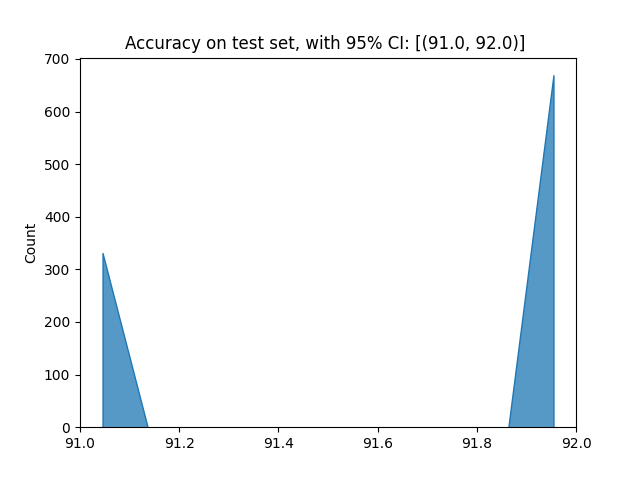
\includegraphics[width=\linewidth]{results/evaluation/logreg_confidence.png}
    \caption{Our best LogRegs performance on 1000 boostrapped test set.}
    \label{fig:C}
\end{figure}

% An appendix can be useful if there are details you want to include that do not fit in the main text. But if you include an appendix, make sure to explicitly refer to it somewhere in the main text.


% ===========================================
\onecolumngrid

\clearpage

\section*{References}
\bibliographystyle{unsrt}
\bibliography{bibliography.bib}


\end{document}